%% For normal draft builds (figs undisplayed hence fast compile)
%\documentclass[hyperpdf,nobind,draft,oneside]{hepthesis}
%\documentclass[hyperpdf,nobind,draft,twoside]{hepthesis}

%% For short draft builds (breaks citations by necessity)
%\documentclass[hyperpdf,nobind,draft,hidefrontback]{hepthesis}

%%For Cambridge soft-bound version
\documentclass[hyperpdf,bindnopdf]{hepthesis}
%% For Cambridge hard-bound version (must be one-sided)
%\documentclass[hyperpdf,oneside]{hepthesis}

%% Load special font packages here if you wish
%\usepackage{lmodern}
\usepackage{mathpazo}
%\usepackage{euler}

%% Put package includes etc. into preamble.tex for convenience
\usepackage{xspace}
\usepackage{tikz}
\usepackage{morefloats,subfig,afterpage}
\usepackage{mathrsfs} % script font
\usepackage{verbatim}

%% Using Babel allows other languages to be used and mixed-in easily
%\usepackage[ngerman,english]{babel}
\usepackage[english]{babel}
\selectlanguage{english}

%% Citation system tweaks
\usepackage{cite}
% \let\@OldCite\cite
% \renewcommand{\cite}[1]{\mbox{\!\!\!\@OldCite{#1}}}

%% Maths
% TODO: rework or eliminate maybemath
\usepackage{abmath}
\DeclareRobustCommand{\mymath}[1]{\ensuremath{\maybebmsf{#1}}}
% \DeclareRobustCommand{\parenths}[1]{\mymath{\left({#1}\right)}\xspace}
% \DeclareRobustCommand{\braces}[1]{\mymath{\left\{{#1}\right\}}\xspace}
% \DeclareRobustCommand{\angles}[1]{\mymath{\left\langle{#1}\right\rangle}\xspace}
% \DeclareRobustCommand{\sqbracs}[1]{\mymath{\left[{#1}\right]}\xspace}
% \DeclareRobustCommand{\mods}[1]{\mymath{\left\lvert{#1}\right\rvert}\xspace}
% \DeclareRobustCommand{\modsq}[1]{\mymath{\mods{#1}^2}\xspace}
% \DeclareRobustCommand{\dblmods}[1]{\mymath{\left\lVert{#1}\right\rVert}\xspace}
% \DeclareRobustCommand{\expOf}[1]{\mymath{\exp{\!\parenths{#1}}}\xspace}
% \DeclareRobustCommand{\eexp}[1]{\mymath{e^{#1}}\xspace}
% \DeclareRobustCommand{\plusquad}{\mymath{\oplus}\xspace}
% \DeclareRobustCommand{\logOf}[1]{\mymath{\log\!\parenths{#1}}\xspace}
% \DeclareRobustCommand{\lnOf}[1]{\mymath{\ln\!\parenths{#1}}\xspace}
% \DeclareRobustCommand{\ofOrder}[1]{\mymath{\mathcal{O}\parenths{#1}}\xspace}
% \DeclareRobustCommand{\SOgroup}[1]{\mymath{\mathup{SO}\parenths{#1}}\xspace}
% \DeclareRobustCommand{\SUgroup}[1]{\mymath{\mathup{SU}\parenths{#1}}\xspace}
% \DeclareRobustCommand{\Ugroup}[1]{\mymath{\mathup{U}\parenths{#1}}\xspace}
% \DeclareRobustCommand{\I}[1]{\mymath{\mathrm{i}}\xspace}
% \DeclareRobustCommand{\colvector}[1]{\mymath{\begin{pmatrix}#1\end{pmatrix}}\xspace}
\DeclareRobustCommand{\Rate}{\mymath{\Gamma}\xspace}
\DeclareRobustCommand{\RateOf}[1]{\mymath{\Gamma}\parenths{#1}\xspace}

%% High-energy physics stuff
\usepackage{abhep}
\usepackage{hepnames}
\usepackage{hepunits}
\DeclareRobustCommand{\arXivCode}[1]{arXiv:#1}
\DeclareRobustCommand{\CP}{\ensuremath{\mathcal{CP}}\xspace}
\DeclareRobustCommand{\CPviolation}{\CP-violation\xspace}
\DeclareRobustCommand{\CPv}{\CPviolation}
\DeclareRobustCommand{\LHCb}{LHCb\xspace}
\DeclareRobustCommand{\LHC}{LHC\xspace}
\DeclareRobustCommand{\LEP}{LEP\xspace}
\DeclareRobustCommand{\CERN}{CERN\xspace}
\DeclareRobustCommand{\bphysics}{\Pbottom-physics\xspace}
\DeclareRobustCommand{\bhadron}{\Pbottom-hadron\xspace}
\DeclareRobustCommand{\Bmeson}{\PB-meson\xspace}
\DeclareRobustCommand{\bbaryon}{\Pbottom-baryon\xspace}
\DeclareRobustCommand{\Bdecay}{\PB-decay\xspace}
\DeclareRobustCommand{\bdecay}{\Pbottom-decay\xspace}
\DeclareRobustCommand{\BToKPi}{\HepProcess{ \PB \to \PK \Ppi }\xspace}
\DeclareRobustCommand{\BToPiPi}{\HepProcess{ \PB \to \Ppi \Ppi }\xspace}
\DeclareRobustCommand{\BToKK}{\HepProcess{ \PB \to \PK \PK }\xspace}
\DeclareRobustCommand{\BToRhoPi}{\HepProcess{ \PB \to \Prho \Ppi }\xspace}
\DeclareRobustCommand{\BToRhoRho}{\HepProcess{ \PB \to \Prho \Prho }\xspace}
\DeclareRobustCommand{\X}{\thesismath{X}\xspace}
\DeclareRobustCommand{\Xbar}{\thesismath{\overline{X}}\xspace}
\DeclareRobustCommand{\Xzero}{\HepGenParticle{X}{}{0}\xspace}
\DeclareRobustCommand{\Xzerobar}{\HepGenAntiParticle{X}{}{0}\xspace}
\DeclareRobustCommand{\epluseminus}{\Ppositron\!\Pelectron\xspace}
\DeclareRobustCommand{\protonproton}{\Pproton\APantiproton\xspace}


%% You can set the line spacing this way
%\setallspacing{double}
%% or a section at a time like this
%\setfrontmatterspacing{double}


%% Define the thesis title and author
\title{GAIT ANALYSIS}
\author{YASH JAIN \\
\centering
under the guidance of \\
Prof. Pranav Nerurkar}

%% Doc-specific PDF metadata
\makeatletter
\@ifpackageloaded{hyperref}{%
\hypersetup{%
  pdftitle = {Studying B to K pi decays with LHCb},
  pdfsubject = {Atharva's PhD thesis},
  pdfkeywords = {LHCb, B, physics, LHC, heavy flavour},
  pdfauthor = {\textcopyright\ Atharva Veer}
}}{}
\makeatother


%% Start the document
\begin{document}

%% Define the un-numbered front matter (cover pages, rubrik and table of contents)
\begin{frontmatter}
  %% Title
\titlepage[of Veermata Jijabai Technical Institute]{%
  A dissertation submitted to the Veermata Jijabai Technical Institute\\ for the degree of Doctor of Philosophy}

%% Abstract
\begin{abstract}%[\smaller \thetitle\\ \vspace*{1cm} \smaller {\theauthor}]
  Gait analysis is the systematic study of animal locomotion, more
specifically the study of human motion, using the eye and the brain of
observers, augmented by instrumentation for measuring body
movements, body mechanics, and the activity of the muscles. Modern gait analysis offers a broad variety of
biomechanical parameters through which to quantify gait. This technique
is widely used in sports industries to analyse the fitness of the athletes. It
can also be used for analyse the motion of the person before and after
any surgery to check the recovery of the patient’s movements.
\end{abstract}


%% Declaration
\begin{declaration}
  This dissertation is the result of my own work, except where explicit
  reference is made to the work of others, and has not been submitted
  for another qualification to this or any other university. This
  dissertation does not exceed the word limit for the respective Degree
  Committee.
  \vspace*{1cm}
  \begin{flushright}
        Yash S Jain
  \end{flushright}
\end{declaration}


%% Acknowledgements
\begin{acknowledgements}
  Of the many people who deserve thanks, some are particularly prominent,
  such as my supervisor\dots
\end{acknowledgements}


%% Preface
\begin{preface}
  This thesis describes my research on various aspects of GAIT Analysis using MPU 8266 and Python.
\end{preface}

%% ToC
\tableofcontents




\end{frontmatter}

%% Start the content body of the thesis
\begin{mainmatter}
  %% Actually, more semantic chapter filenames are better, like "chap-bgtheory.tex"
  \chapter{MPU 6050}
\label{chap:SomeStuff}

%% Restart the numbering to make sure that this is definitely page #1!
\pagenumbering{arabic}

%% Note that the citations in this chapter use the journal and
%% arXiv keys: I used the SLAC-SPIRES online BibTeX retriever
%% to build my bibliography. There are also quite a few non-standard
%% macros, which come from my personal collection. You can have them
%% if you want, or I might get round to properly releasing them at
%% some point myself

The MPU-6050 parts are the world’s first MotionTracking devices
designed for the low power, low cost, and high-performance requirements
of smartphones, tablets and wearable sensors.

SThe MPU-6050 incorporates InvenSense’s MotionFusion and run-time
calibration firmware that enables manufacturers to eliminate the costly
and complex selection, qualification, and system level integration of
discrete devices in motion-enabled products, guaranteeing that sensor
fusion algorithms and calibration procedures deliver optimal performance
for consumers.

The MPU-6050 devices combine a 3-axis gyroscope and a 3-axis
accelerometer on the same silicon die, together with an onboard Digital
Motion Processor (DMP), which processes complex 6-axis MotionFusion
algorithms. The device can access external magnetometers or other
sensors through an auxiliary master I2C bus, allowing the devices to
gather a full set of sensor data without intervention from the system
processor. The devices are offered in a 4 mm x 4 mm x 0.9 mm QFN
package.
  \chapter{IMPLEMENTATION (using MPU-6050)}
\label{chap:MoreStuff}

\section{Implementation}
MPU-6050 was connected to the Wemos board as shown in the above
pin diagram. SCL and SDA pins are used for sending data via I2C
communication protocol.

Using Ardunio IDE we programmed Wemos Board to get accelerometer
and gyroscope data.

Accelerometer data had gravity component in all three axes which is
undesirable and so we filtered that out using a low pass filter by applying
the following transformation on all three axes.
g = 0.9 * g + 0.1 * v
Where g is a global variable initialized to 0 and v is accelerometer reading
of any axis.

7

Using v = v – g you can remove the gravity factor in that axis.
Time interval between two readings was calculated using the difference
in the times in milliseconds returned by the millis() function in the Ardunio
library.

We created a local server using XAMPP and using ESP8266 we uploaded
the MPU data using PHP to MySQL database that was hosted on the local
server.

Once the data was uploaded using the server then the data from the local
server was fetched using python library MySQLdb. We then applied
complementary filters on the raw data to remove noise.

We initially tried to interpolate the accelerometer readings using the
interpolate function in SciPy module. But the results of the plot and time
taken to plot was not at all satisfactory so we then used the Simpson’s
Method of integration using the simps() function in the scipy.integrate
module. Using this we integrated the acceleration data twice with respect
to time to get displacement.

Finally after receiving the displacements in all 3 directions, we used
matplotlib.pyplot to get the 3D graph of the motion.

\section{Problems Faced}
As mentioned above, the MPU-6050 is a cheap module and thus
generates a lot of noise in the data. While, for a lot of applications this
noise can be filtered effectively and the MPU-6050 can be used
satisfactorily, but in our case even the slightest of noise got magnified over
and over again as we integrated over large time intervals.

8
As a result we always got a increasing or decreasing displacement
irrespective of the motion performed because the errors kept on adding
up.

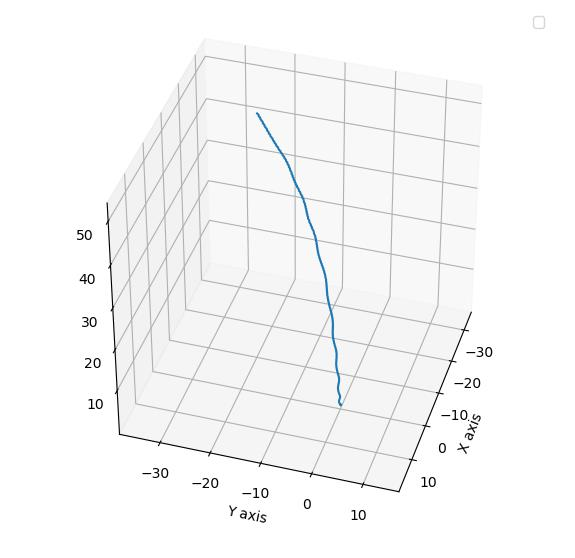
\includegraphics[width=10cm]{plot.png}

  %% To ignore a specific chapter while working on another, making the build faster, comment it out:
  %\input{chap4}
\end{mainmatter}

%% Produce the appendices
\begin{appendices}
  

\end{appendices}

%% Produce the un-numbered back matter (e.g. colophon,
%% bibliography, tables of figures etc., index...)
\begin{backmatter}
  \chapter{Conclusion}

%% Restart the numbering to make sure that this is definitely page #1!
\pagenumbering{arabic}

%% Note that the citations in this chapter use the journal and
%% arXiv keys: I used the SLAC-SPIRES online BibTeX retriever
%% to build my bibliography. There are also quite a few non-standard
%% macros, which come from my personal collection. You can have them
%% if you want, or I might get round to properly releasing them at
%% some point myself

Thus, from the above plots we can conclude that the MPU-6050 is very
inferior compared to Mobile Phone Sensors and hence, MPU-6050 cannot
be used for reliable position tracking.

Also, while the plots using Mobile Phone Sensors are quite good for the
above datasets, we need to take into account the fact that these datasets
are for motions performed in small time intervals only. For larger time
intervals, even the Mobile Sensors was not able to give us satisfactory
results.

Thus the Conclusion of this project is that pure IMU based position
tracking is infeasible and for accurate results we always require optical
sensors and cameras. But for smaller datasets and a cheaper alternative,
IMU based position tracking can prove to be useful.

%% You're recommended to use the eprint-aware biblio styles which
%% can be obtained from e.g. www.arxiv.org. The file mythesis.bib
%% is derived from the source using the SPIRES Bibtex service.
\bibliographystyle{h-physrev}
\begin{thebibliography}{}

\bibitem{rand}
\\\texttt{https://matplotlib.org/1.4.2/users/pyplot_tutorial.html}

\bibitem{rand2}
\\\texttt{https://docs.scipy.org/doc/scipy/reference/tutorial/integrate.html}

\bibitem{rand3}
\\\texttt{https://docs.scipy.org/doc/scipy/reference/interpolate.html}

\bibitem{rand4}
\\\texttt{https://pykalman.github.io/}

\bibitem{rand5}
\\\texttt{http://mysql-python.sourceforge.net/MySQLdb.html}

\bibitem{rand6}
\\\texttt{http://www.starlino.com/imu_guide.html}

\end{thebibliography}


%% I prefer to put these tables here rather than making the
%% front matt

%% If you have time and interest to generate a (decent) index,
%% then you've clearly spent more time on the write-up than the 
%% research ;-)
%\printindex

\end{backmatter}

%% Close
\end{document}
